\chapter{Plbmng Tool}
\label{chapter:plbmng}
Plbmng application called \texttt{Data miner for PlanetLab} is available at public PyPi repository\footnote{PyPi page of the plbmng tool: https://pypi.org/project/plbmng/}. The tool allows managing \texttt{PlanetLab} nodes, gathering information about them and pulling the latest data from the \texttt{PlanetLab} API service. Its core is written in Bash and additional modules are written in Python 3 \cite{suba1}. At the moment, it is depended on both Bash and Python modules and it's installation consists of several steps:
\begin{itemize}
	\item Installing the application from PyPi repository or downloading the source codes from GitHub.
	\item Installing additional system packages like dialog,pssh and fping.
	\item Locating installation folder and putting symlink into \texttt{\$PATH} directory.
\end{itemize}
After the first start of the application user is required to fill credentials and \texttt{SSH} public key details to be able to access 	exttt{PlanetLab} API and nodes using the menu option \texttt{Credentials}. All the current options in the menu are \texttt{Search nodes} for retrieving a node from internal database, \texttt{Measure Menu} that allows user to schedule gathering of data about the nodes or run the data gathering now, \texttt{Map Menu} that allow user to generate map showing location of the nodes and mentioned \texttt{Settings}. Menu is created using bash library \texttt{dialog} and can be seen in Figure~\ref{fig:planetlaboldmenu}. 

\begin{figure}[H]
	\centering
	\scalebox{0.4}{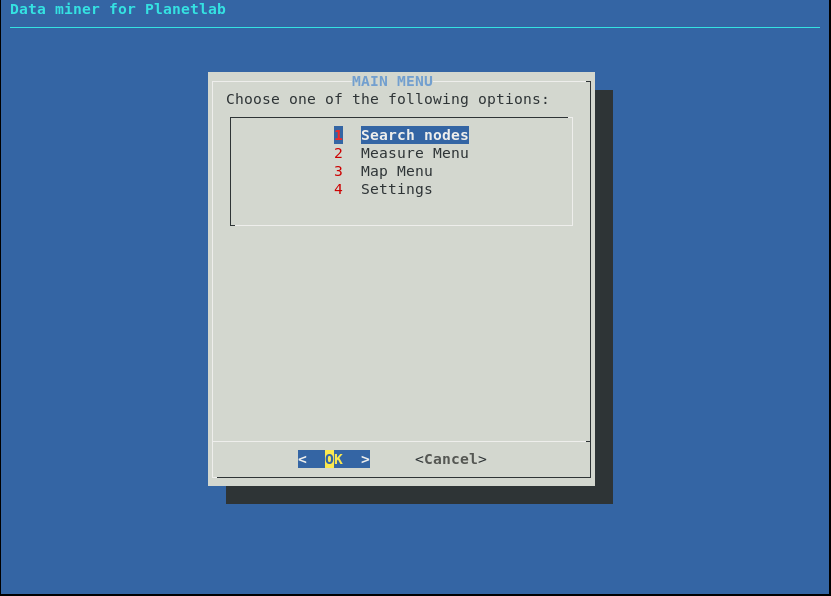
\includegraphics{obrazky/planetlabmenuold}}
	\caption{Data miner for PlanetLab menu.}
	\label{fig:planetlaboldmenu}
\end{figure}

asd
\section{Current Tool Funcionality}

\section{Current Tool State}
The first problem of the existing tool is language disparity having half of the functionality in Bash and half of the functionality in Python 3. This makes it difficult to make adjusment to the tool as one needs to study a great amount of scripts that are in several different folders. 
\section{Areas of improvement}
easier installation
description of the menu
\chapter{	exttt{PlanetLab} Network}
\label{chapter:	exttt{PlanetLab}network}

\chapter{Linux and Virtualization}
\label{chapter:Linux}

\chapter{Plbmng Tool Improvements}
\label{chapter:improve}

Teoretické zázemí studentské práce vhodně rozdělené do částí.

(Struktura navržená v~této šabloně je nejhrubší možná, po konzultaci s~vedoucím je vhodné zvolit přiléhavější.)
